%%%%%%%%%%%%%%%%%%%%%%%%%%%%%%%%%%%%%%%%%%%%%%%%%%%%%%%%%%%%%%%%%%%%%%%%%%%%%%%%%%%%
% Do not alter this block (unless you're familiar with LaTeX)
\documentclass{../labbook}
\usepackage{booktabs}
\usepackage{siunitx}
\usepackage{multirow}
\usepackage{adjustbox}
%%%%%%%%%%%%%%%%%%%%%%%%%%%%%%%%%%%%%%%%%%%%%
%Fill in the appropriate information below
\lhead{Group lab 2}
\rhead{Speech Sounds} 
\chead{\textbf{ Due: \textbf{WED 18.10.2023 23:59} CEST}}
%%%%%%%%%%%%%%%%%%%%%%%%%%%%%%%%%%%%%%%%%%%%%

\begin{document}
\begin{mdframed}[backgroundcolor=blue!20]
\LaTeX ~submissions are mandatory. Submitting your assignment in another format will be graded no higher than R.
\end{mdframed}

%%%%%%%%%%%%%%%%%%%%%%%%%%%%%%
\section{Group members}
Cantao Su, Chenyu Li, Weihao Jiang, Yanhua Liao
%%%%%%%%%%%%%%%%%%%%%%%%%%%%%%

\section{In-class lab 2.}
In this group lab we will be exploring emotional speech. For this we will take a subset from the audio portion of the \href{https://www.kaggle.com/uwrfkaggler/ravdess-emotional-speech-audio/}{Ryerson Audio-Visual Database of Emotional Speech and Song} (RAVDESS\footnote{https://doi.org/10.1371/journal.pone.0196391}). Overall, tthere are 1440 files (60 trials per actor x 24 actors = 1440). 
The RAVDESS contains 24 professional actors (12 female, 12 male) vocalizing two lexically-matched statements in a neutral North American accent. Speech emotions includes calm, happy, sad, angry, fearful, surprise, and disgust expressions. 
Each expression is produced at two levels of emotional intensity (normal, strong), with an additional neutral expression.

Speech emotions include calm, happy, sad, angry, fearful, surprise, and disgust expressions. Each expression is produced at two levels of emotional intensity (normal, strong), with an additional neutral expression.

The filename consists of a 7-part numerical identifier (e.g., 03-01-06-01-02-01-12.wav). These identifiers define the stimulus characteristics (in bold - those characteristics that are relevant for this lab):
\begin{itemize}
    \item Modality (01 = full-AV, 02 = video-only, \textbf{03 = audio-only}).
    \item Vocal channel (\textbf{01 = speech}, 02 = song).
    \item Emotion (\textbf{01 = neutral}, 02 = calm, \textbf{03 = happy}, \textbf{04 = sad}, \textbf{05 = angry}, \textbf{06 = fearful}, 07 = disgust, \textbf{08 = surprised}).
    \item Emotional intensity (01 = normal, \textbf{02 = strong}). NOTE: There is no strong intensity for the 'neutral' emotion.
    \item Statement (01 = "Kids are talking by the door", \textbf{02 = "Dogs are sitting by the door"}). 
    \item Repetition (01 = 1st repetition, 02 = 2nd repetition).
    \item Actor (01 to 24. Odd numbered actors are male, even numbered actors are female).
\end{itemize}

We will be exploring a small subset of recordings: 10 actors, one trial in neutral state (no emotion) and in five different emotions (anger, fear, happiness, sadness, surprise).

We will explore several simple measurements related to prosody and see if the results tell us anything and if our perceptual observations are comparable. 


\subsubsection*{Preparation:}
For your group lab you will need:
\begin{itemize}
    \item Decide which of the four emotions above you would like to explore.
    \item Take the recordings of the neutral state speech and the emotional state speech (in the emotion you have chosen) from \href{https://drive.google.com/drive/folders/11jGlJaEVkZL6PLsL-Si8RY4DbsP409JC?usp=sharing}{here}.
\end{itemize}

\begin{problem}{1}{10}{Simple prosody measurements in emotional speech}
We will look into several simple \textbf{measurements} that relate to fundamental frequency (f0) and rate:

\begin{enumerate}
    \item Speech rate (number of syllables / total time) - use either \href{https://sites.google.com/site/speechrate/speech-rate-praat-script-that-detects-syllable-nuclei/praat-script-syllable-nuclei-v2}{this script by Nivja de Jong and Ton Wempe (2009)}, or the \href{https://sites.google.com/view/uhm-o-meter}{its newer version}, you can find tutorials and descriptions on the website as well.
    \item Articulation rate (number of syllables / phonation time) - use the same script.
    \item In Praat: mean f0 over the whole phrase (select phrase – ``Pitch -> get pitch''), you can also do that with your own R/Python script.
    \item In Praat: f0 range in the whole phrase  (select phrase – ``Pitch -> get pitch maximum'' and ``get pitch minimum'', and based on that calculate range), you can also do that with your own R/Python script.
    \item f0 variance, average of the squared deviations from the mean of f0: 
$var = mean | f0 - mean (f0)|^2$  (select phrase -- ``get pitch listing'', 
save as text file, clean it to keep only the numbers, calculate according to the formula. You can use Python, R, excel – whatever you wish \footnote{Python hint: 

		$f0 = np.array(f0)$
  
		$m = np.mean(f0)$ 
  
		$v = np.mean((f0 - m)**2) )$ })

   
\end{enumerate}

\subsubsection*{Task:}

\begin{enumerate}
    \item Listen to the recordings you selected to work with. 
    \item Together with your group members, hypothesize which of the given measurement(s) could work best to differentiate between recordings of neutral and emotional speech.
    \item Calculate all the measurements listed above for every recording (you should get 50 measured values for neutral speech and 50 measured values for emotional speech).
    \item In your answer, report how you obtained the measurements and any difficulties you have faced in the process.
    \item Calculate simple descriptive statistics (mean, median and standard deviation) and visualize the measurements (for example with a box plot) to compare neutral and emotional speech. There is no need to calculate descriptive statistics or plot anything per individual speaker.
    \item Include the descriptive statistics and plots in your LaTeX report (see the previous lab book for an example of '\texttt{includegraphics}').
    \item For each measurement describe the differences you see between neutral state and emotional state measurements you see (if there are any).
    \item Has your hypothesis about the measurements from step 2 been confirmed? If not, what other measurement (if any) was the best for the differentiation between recordings of neutral and emotional speech?
\end{enumerate}

\end{problem}

%%%%%%%%%%%%%%%%%%%%%%%%%%%%%%%%%%%%%%%%%%%%%
\begin{solution}

\subsubsection{Your hypothesis, steps 1-2}

In these datasets, we posit that \underline{\textbf{speech rate}} serves as the most telling indicator of emotional shifts during moments of anger. Drawing from personal experiences and observations, when individuals find themselves in a state of anger or embroiled in a heated argument, their speech rate tends to exhibit a discernible uptick. For instance, sentences may flow out more rapidly, with phrases strung together in quick succession, and there is often a dearth of pauses or hesitations, as if the words rush forth unimpeded by self-regulation. This heightened speech rate can be likened to a verbal storm, reflecting the turbulence of emotions experienced during such moments of intense irritation or rage.

\subsubsection{Measurements, descriptive statistics and plots, steps 3-6}

\begin{figure}[h!]
    \centering
    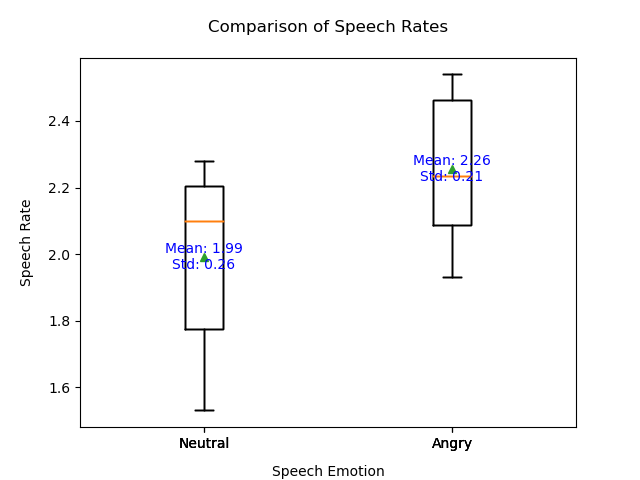
\includegraphics[width=0.7\textwidth]{1stM.png}
    \caption{Comparison of Speech Rates for Neutral ($median=2.1, mean=1.99, sd=0.26$) and Angry ($median=2.2,mean=2.26, sd=0.21$)}
\end{figure}

\begin{figure}[!h]
    \centering
    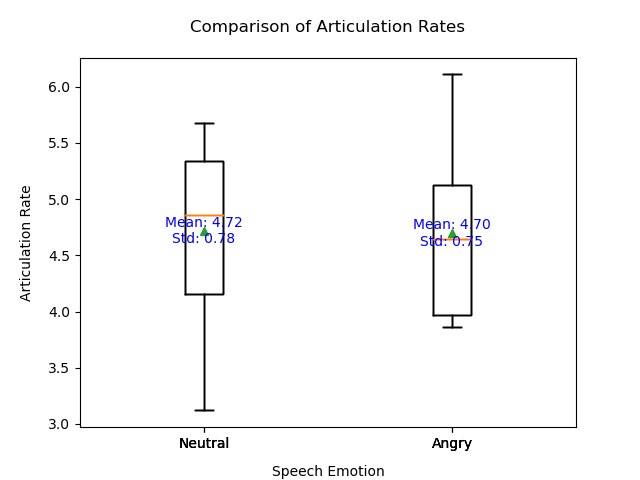
\includegraphics[width=0.7\textwidth]{2ndM.png}
    \caption{Comparison of Articulation Rates for Neutral ($median=4.9, mean=4.72, sd=0.78$) and Angry ($median=4.6, mean=4.70, sd=0.75$)}
\end{figure}

\begin{figure}[!h]
    \centering
    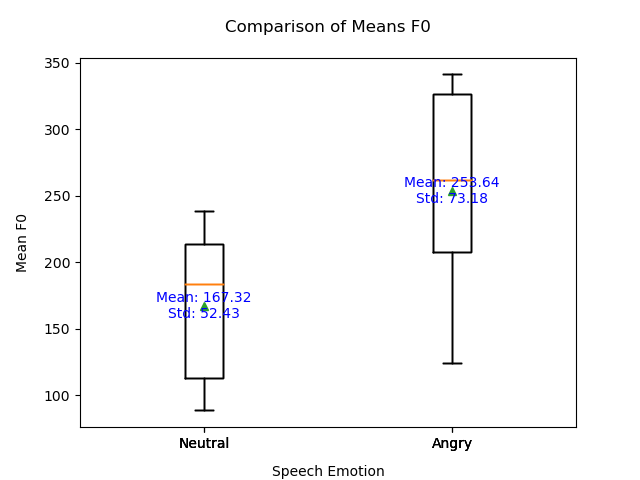
\includegraphics[width=0.7\textwidth]{3rdM.png}
    \caption{Comparison of Means F0 for Neutral ($median=183.3, mean=167.32, sd=52.43$) and Angry ($median=261.7, mean=253.64, sd=73.18$)}
\end{figure}

\begin{figure}[!h]
    \centering
    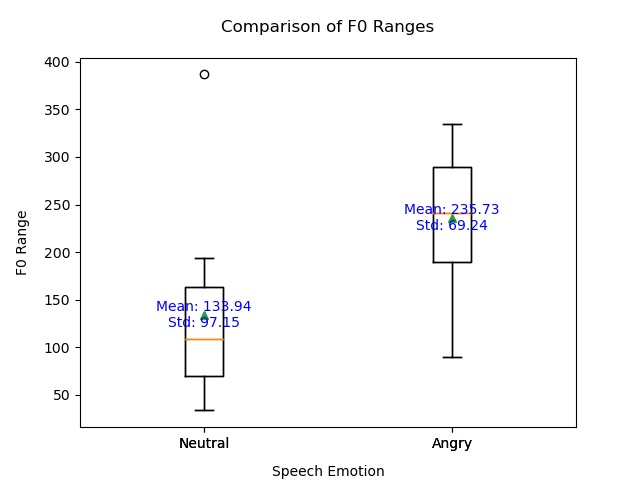
\includegraphics[width=0.7\textwidth]{4thM.png}
    \caption{Comparison of f0 variance for Neutral ($median=109.1, mean=133.94, sd=97.15$) and Angry ($median=241.0, mean=235.73, sd=69.24$)}
\end{figure}

\begin{figure}[!h]
    \centering
    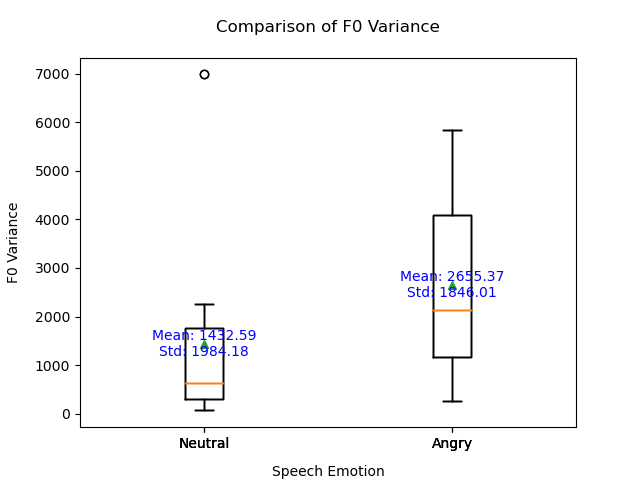
\includegraphics[width=0.7\textwidth]{5thM.png}
    \caption{Comparison of f0 variance for Neutral ($median=628.5, mean=1432.59, sd=1984.18$) and Angry ($median=2136.2, mean=2655.37, sd=1846.01$)}
\end{figure}

\begin{table}
    \centering
    \adjustbox{max width=\textwidth}{
    \begin{tabular}{cccccccccccc}
    \toprule
    \multirow{2}{*}{Measurements} & \multicolumn{2}{c}{Speech Rate} & \multicolumn{2}{c}{Articulation Rate} & \multicolumn{2}{c}{Mean F0} & \multicolumn{2}{c}{F0 Range} & \multicolumn{2}{c}{F0 Variance}\\
    \cmidrule(lr){2-3} \cmidrule(lr){4-5} \cmidrule(lr){6-7} \cmidrule(lr){8-9} \cmidrule(lr){10-11}
    & Neutral & Angry & Neutral & Angry  & Neutral & Angry & Neutral & Angry & Neutral & Angry \\
    \midrule
    Aud. 1 & 1.50 & 2.10 & 4.00 & 4.10 & 112.30 & 258.20 & 60.00 & 180.30 & 245.30 & 4315.70 \\
    Aud. 2 & 2.30 & 2.00 & 5.60 & 3.90 & 115.00 & 157.50 & 70.70 & 218.20 & 2253.40 & 5200.60 \\
    Aud. 3 & 2.20 & 2.50 & 5.10 & 6.10 & 238.70 & 218.50 & 193.70 & 233.30 & 6982.80 & 2427.00 \\
    Aud. 4 & 1.70 & 2.50 & 4.10 & 5.60 & 176.60 & 123.90 & 386.80 & 89.60 & 2090.70 & 3443.40 \\
    Aud. 5 & 2.20 & 1.90 & 5.70 & 3.90 & 215.10 & 204.60 & 173.40 & 177.10 & 286.60 & 5837.30 \\
    Aud. 6 & 2.00 & 2.30 & 4.60 & 4.30 & 218.10 & 341.30 & 120.90 & 334.50 & 789.00 & 1110.70 \\
    Aud. 7 & 1.60 & 2.50 & 3.10 & 5.20 & 110.20 & 339.90 & 68.80 & 293.20 & 352.90 & 1845.30 \\
    Aud. 8 & 2.30 & 2.20 & 5.40 & 3.90 & 189.90 & 265.30 & 134.10 & 277.60 & 606.00 & 1340.00 \\
    Aud. 9 & 2.20 & 2.40 & 5.20 & 5.00 & 88.60 & 339.60 & 33.60 & 248.70 & 68.40 & 266.20 \\
    Aud. 10 & 1.90 & 2.20 & 4.40 & 5.00 & 208.60 & 287.70 & 97.40 & 304.80 & 650.90 & 767.50 \\
    Mean & 2.00 & 2.30 & 4.70 & 4.70 & 167.30 & 253.60 & 133.90 & 235.70 & 1432.60 & 2655.40 \\
    Median & 2.10 & 2.20 & 4.90 & 4.60 & 183.30 & 261.70 & 109.10 & 241.00 & 628.50 & 2136.20 \\
    SD & 0.26 & 0.21 & 0.78 & 0.75 & 52.43 & 73.18 & 97.15 & 69.24 & 1984.18 & 1846.01 \\
    \bottomrule
    \end{tabular}
    }
    \caption{Table with Subheaders}
\end{table}

\subsubsection{(Visual) analysis of the measurements and conclusions, steps 7-8}

\paragraph{Analysis of Measurements:\\} 

Analyzing the box plots of \underline{\textbf{speech rate}}, we observe that the descriptive statistics for the two emotions are quite close. However, there are slight differences in the mean and median values, with anger exhibiting slightly higher rates. Furthermore, the standard deviation for the neutral condition is marginally greater, though the disparities are relatively minor. Notably, the anger condition also features a higher maximum value.

Turning our attention to the \underline{\textbf{articulation rate}} plot, we note that the median, mean, and standard deviation values are in close proximity. Nevertheless, there are distinct disparities in the maximum and minimum values, especially with regards to the minimum value. The articulation rate for the angry condition is notably higher than that for the neutral condition.

Upon examining the \underline{\textbf{mean F0}} plot, a substantial variance among the various indicators becomes apparent. The mean and median values for the angry condition are significantly elevated by approximately 100Hz compared to the neutral condition. In contrast, the standard deviation for the neutral condition undergoes a marked reduction in comparison to the angry state. While the minimum values for both conditions are nearly identical, the maximum value for the angry condition is 100Hz higher.

Analyzing the \underline{\textbf{F0 range}} chart reveals a pattern consistent with the preceding mean F0 findings. Notably, the interquartile range, which signifies the frequency range between the upper and lower quartiles, appears to be narrower, indicating that the F0 range for each instance of anger is relatively concentrated. This phenomenon could be attributed to the inclusion of both male and female voices in the audio, as women typically exhibit higher F0 values and a broader vocal range. This factor contributes to the expansion of the maximum mean F0 value.

In the context of the \underline{\textbf{F0 variance}} box plot, substantial disparities exist between the mean and median values for both the neutral and angry emotional states, with deviations exceeding 1000 Hz. It's worth noting that the standard deviation of the neutral state is greater than that of the angry state. Furthermore, the interquartile range for the angry state is notably broader compared to the neutral state. Even when considering their minimum values, the range for F0 variance in the angry state is nearly twice that of the neutral state.

\paragraph{Conclusions of Hypothesis:\\å}

Our data clearly demonstrates a significant difference in the fundamental frequency range (F0 range) between the emotions of anger and neutrality. \underline{The fundamental frequency (F0)} \underline{is a crucial acoustic parameter in sound waveforms that represents pitch variations.}

In the context of anger, speech typically becomes impulsive and less controlled. This impulsivity can lead to a reduction in the smoothness of speech, resulting in rapid and emotionally charged articulation. These factors collectively impact the fundamental frequency (F0), leading to frequent fluctuations in F0.

Anger is often accompanied by intense emotional expression. When individuals are angry, they tend to express themselves with heightened emotion, resulting in noticeable changes in pitch. Elevated pitch, characterized by high or rapid tonal variations, serves to emphasize the intensity of anger. Consequently, F0 tends to significantly increase to convey the emotional fervor.

Furthermore, increased muscular tension in the face and throat is a common occurrence during anger. This heightened tension affects the vibration of the vocal cords, causing a rise in pitch. The combination of high pitch and tense vocalization may lead to rapid fluctuations in the frequency of vocal cord vibrations, further increasing F0.

In summary, the observable variations in F0 during states of anger can be attributed to the demand for emotional expression, physiological changes in vocal cord tension, and alterations in speech fluency. The uncontrolled and rapid nature of speech during anger can result in frequent F0 fluctuations, collectively serving as a distinctive marker of this emotional state.
\end{solution}

%%%%%%%%%%%%%%%%%%%%%%%%%%%%%%%%%%%%%%%%%%%%%



\bigskip
\textbf{References}:

\noindent De Jong, N.H. \& Wempe, T. (2009). Praat script to detect syllable nuclei and measure speech rate automatically. Behavior research methods, 41 (2), 385 - 390. 

De Jong, N.H., Pacilly, J., \& Heeren, W. (2021). PRAAT scripts to measure speed fluency and breakdown fluency in speech automatically, Assessment in Education: Principles, Policy \& Practice, 28:4, 456-476, DOI: 10.1080/0969594X.2021.1951162 

\end{document}
